%%%%%%%%%%%%%%%%%%%%%%%%%%%%%%%%%%%%%%%%%
% Short Sectioned Assignment
% LaTeX Template
% Version 1.0 (5/5/12)
%
% This template has been downloaded from:
% http://www.LaTeXTemplates.com
%
% Original author:
% Frits Wenneker (http://www.howtotex.com)
%
% License:
% CC BY-NC-SA 3.0 (http://creativecommons.org/licenses/by-nc-sa/3.0/)
%
%%%%%%%%%%%%%%%%%%%%%%%%%%%%%%%%%%%%%%%%%

%----------------------------------------------------------------------------------------
%   PACKAGES AND OTHER DOCUMENT CONFIGURATIONS
%----------------------------------------------------------------------------------------

\documentclass[paper=a4, fontsize=11pt]{scrartcl} % A4 paper and 11pt font size

\usepackage[T1]{fontenc} % Use 10-bit encoding that has 256 glyphs
\usepackage{polski}
\usepackage[utf8]{inputenc}
\usepackage[polish]{babel}
\usepackage{amsmath,amsfonts,amsthm} % Math packages
\usepackage{pgfplots} % Math packages
\usepackage{lipsum} % Used for inserting dummy 'Lorem ipsum' text into the template
\usepackage{enumerate}
\usepackage{sectsty} % Allows customizing section commands
\usepackage{fancyhdr} % Custom headers and footers
\usepackage{listings}


\pagestyle{fancyplain} % Makes all pages in the document conform to the custom headers and footers
\fancyhead{} % No page header - if you want one, create it in the same way as the footers below
\fancyfoot[L]{} % Empty left footer
\fancyfoot[C]{} % Empty center footer
\fancyfoot[R]{\thepage} % Page numbering for right footer
\renewcommand{\headrulewidth}{0pt} % Remove header underlines
\renewcommand{\footrulewidth}{0pt} % Remove footer underlines
\setlength{\headheight}{13.6pt} % Customize the height of the header
\usepackage{listings}

\pgfplotsset{compat=1.10}
\numberwithin{equation}{section} % Number equations within sections (i.e. 1.1, 1.2, 2.1, 2.2 instead of 1, 2, 3, 4)
\numberwithin{figure}{section} % Number figures within sections (i.e. 1.1, 1.2, 2.1, 2.2 instead of 1, 2, 3, 4)
\numberwithin{table}{section} % Number tables within sections (i.e. 1.1, 1.2, 2.1, 2.2 instead of 1, 2, 3, 4)

\setlength\parindent{0pt} % Removes all indentation from paragraphs - comment this line for an assignment with lots of text

%----------------------------------------------------------------------------------------
%   TITLE SECTION
%----------------------------------------------------------------------------------------

\newcommand{\horrule}[1]{\rule{\linewidth}{#1}} % Create horizontal rule command with 1 argument of height

\title{ 
    \normalfont \normalsize 
    \textsc{Politechnika Warszawska} \\ [25pt] % Your university, school and/or department name(s)
    \horrule{0.5pt} \\[0.4cm] % Thin top horizontal rule
    \huge Testowanie i weryfikacja oprogramowania Zadanie projektowe: Łańcuch odpowiedzialności\\ % The assignment title
    \horrule{2pt} \\[0.5cm] % Thick bottom horizontal rule
}

\author{Mateusz Starzycki} % Your name

\date{\normalsize\today} % Today's date or a custom date

\begin{document}

\maketitle % Print the title

%----------------------------------------------------------------------------------------
%   PROBLEM 1
%----------------------------------------------------------------------------------------

\newpage

\section{Wprowadzenie}


Celem zadania było opracowanie wzorca projektowego łańcuch odpowiedzialności.
Wzorzec ten jest wzorcem behewioralnym. W przypadku w którym zapytanie ma zostać obsłużone
jest ono kierowane do klasy łańcucha odpowiedzialności, następnie wszystkie, połączone w
łańcuch klasy sprawdzają czy potrafią dane zachowanie obsłużyć, w przypadku gdy jest to możliwe,
pierwsza klasa potrafiąca wykonać zadanie wykonuje je.

Warto zauważyć iż istnieje możliwość przejścia przez cały łańcuch odpowiedzialności i porzucenie
zadania w przypadku gdy żadna z klas nie będzie potrafiła poradzić sobię z zadaniem.

\section{Opis implementacji}

Implementacja została wykonana w następujący sposób:

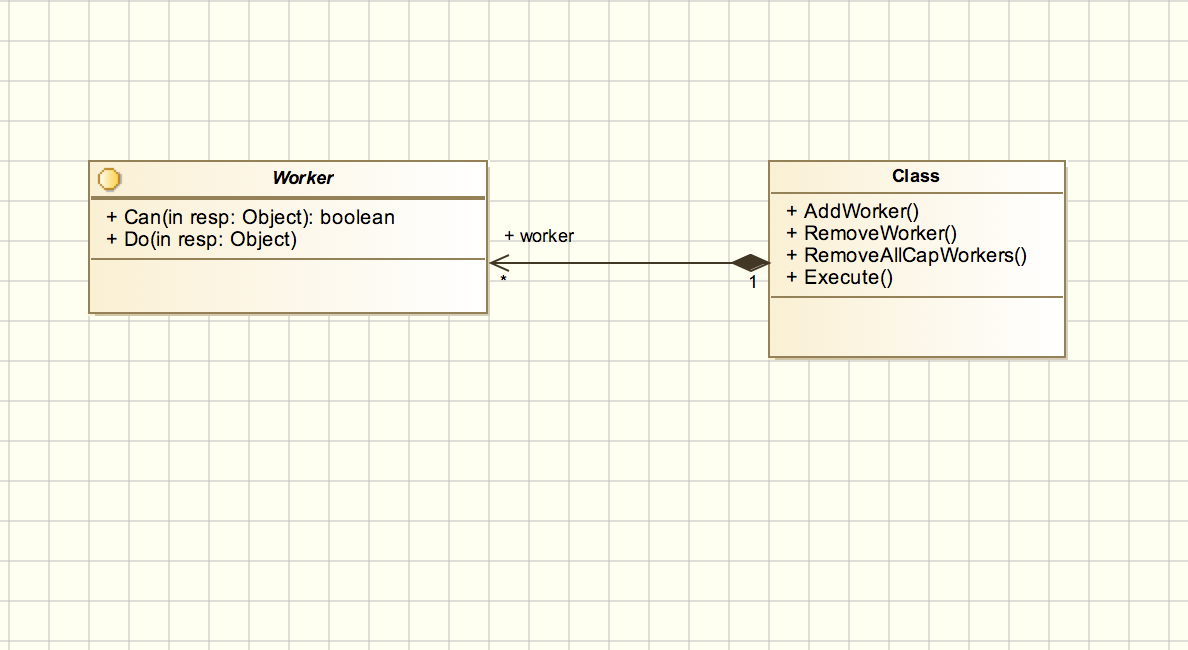
\includegraphics[width=\textwidth]{5}

Klasa chain of responsibilities jest to abstrakcyjna klasa o publicznym interfejsie worker.
Interfejs worker służy do implementacji wykonującej pracę klasy. Zadaniem korzystającego z klasy
jest zdefiniowanie odpowiedzialności workerów oraz ułożenie odpowiedniej struktury klas przekazywanych
do nich. Sama odpowiedzialność systemu przekazywana jest do workerów przy pomocy obiektu podstawowego
javy - Object. Daje to możliwość ewentualnej introspekcji obiektu oraz nie narzuca żadnych kryteriów
co do struktury hierarchi klas w programie.


\section{Dokumentacja Użytkownika}


W celu skorzystania z klasy chain of responsibility należy rozpocząć od napisania klas typu worker.
Klasy te muszą implementować wirtualne metody can oraz do.

Metod can o sygnaturze \(boolean Can(Object resp)\) służy do określenia czy dany worker może wykonać
zadanie mu powierzone, funkcja zwraca prawde w przypadku gdy zapytanie może zostać wykonane, fałsz 
w innym przypadku.
Metoda do o sygnaturze \(void Do (Object resp)\) wykonuje pracę dla obiektu resp.

Przykładowa implementacja klas:

\lstinputlisting[language=Java]{tworzcor.java}

Sama implementacja klasy nie jest wystarczająca do skorzystania z klasy chain of responsiblity.
W celu przypisania objektów typu worker, należy utworzyć ich obiekty oraz dodać ich do obiektu klasy
chain of responsibility.

W tym celu należy stworzyć klasę chain of responsibility (lub jej potomka):

\lstinputlisting[language=Java]{dodaj.java}

Po utworzeniu oraz dodaniu workerów do klasy funkcja execute powinna automatycznie wykonać powierzoną 
odpowiedzialność.

Dodatkowymi funkcjami dla użytkownika są - usunięcie wybranego workera (RemoveWorker) oraz usunięcie
wszystkich workerów potrafiących wyknać daną odpowiedzialność (RemoveAllCapableWorker).

\section{Planowanie testów}

Testy podzielono na testy biało oraz czarno skrzynkowe. Nie ma sensu testowania integreacyjnego
gdyż program składa się z jednej klasy. Z powodu ograniczonego czasu na pisanie projektu nie napisano
jako takich testów wydajnościowcyh, motywowane to także było prostotą pisanego rozwiazania, jedynym
czasochłonnym zadaniem w przypadku klasy Chain of responsibility jest przeszukiwanie listy workerów. Jest
to jednak zadanie liniowe i w przypadku implementacji dostarczonej klientowi założono iż łańcuchy te nie będą
długie, skomplikowane mogą być natomoiast workery wyjkonujące zadania.

Testy czarno skrzynkowe ze względu na ograniczoną przez wąski interfejs ilością możliwości interakcji z
systemem zaprojektowano jako następujące testy:
\begin{itemize}
  \item Test dodania i usunięcia workera
  \item Test wykonania workerów
  \item Test wykonania dla braku odpowiedniego workera
  \item Próba usunięcia nieistniejącego workera
  \item Próba wielokrotnego dodania tego samego workera
  \item Próba usunięcia workera wielokrotnie
\end{itemize}

Kolejnym etapem były testy białoskrzynkowe, właściwie był to proces adaptacji istniejących testów czarno skrzynkowych
w celu sprawdzenia pokrycia wszystkich węzłów w grafach.

\section{Testy czarnoskrzynkowe }

Na podstawie opisanej dokumentacji zostały stworzone testy czarno skrzynkowe implementujące klasę
worker oraz chain of responsibility. Podczas testowania użyto trywialnych przykładów zwracających zawsze
prawde, oraz takich które wykonywały zapytanie jedynie dla wybranego łańcucha znaków.

Testy zostały zakończone po uzyskaniu pozytywnych wyników.


\section{Testy białoskrzynkowe }

Pierwszym krokiem testów białoskrzynkowych była analiza funkcji systemu.
Sporządzono diagramy wszystkich funkcji klasy Chain of responsibility:

Diagram dla RemoveAllCapableWorker:

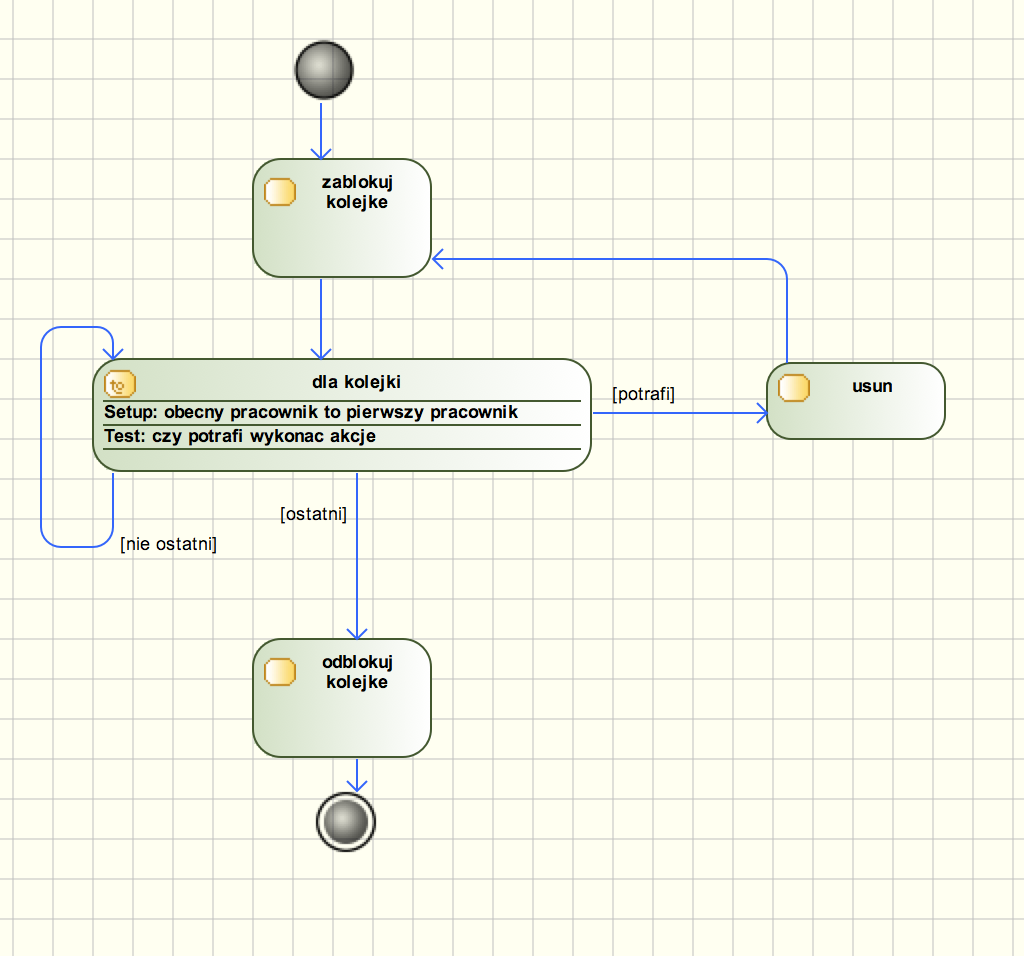
\includegraphics[width=\textwidth]{1}

Diagram dla RemoveWorker:

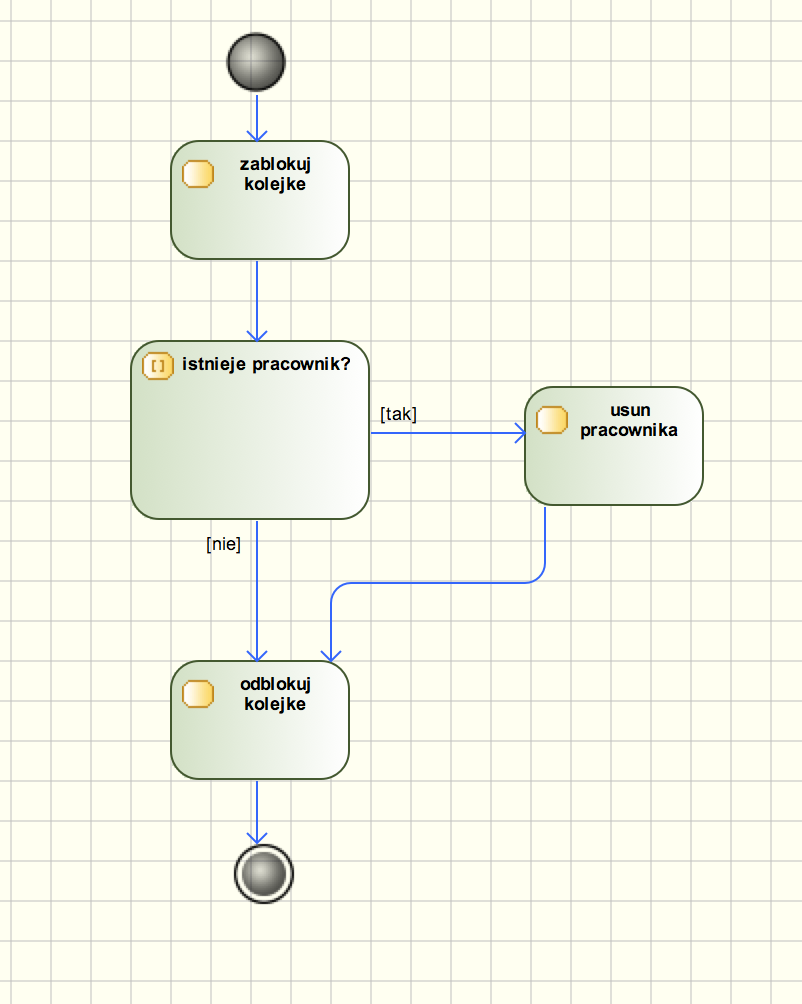
\includegraphics[width=\textwidth]{2}

Diagram dla Execute:

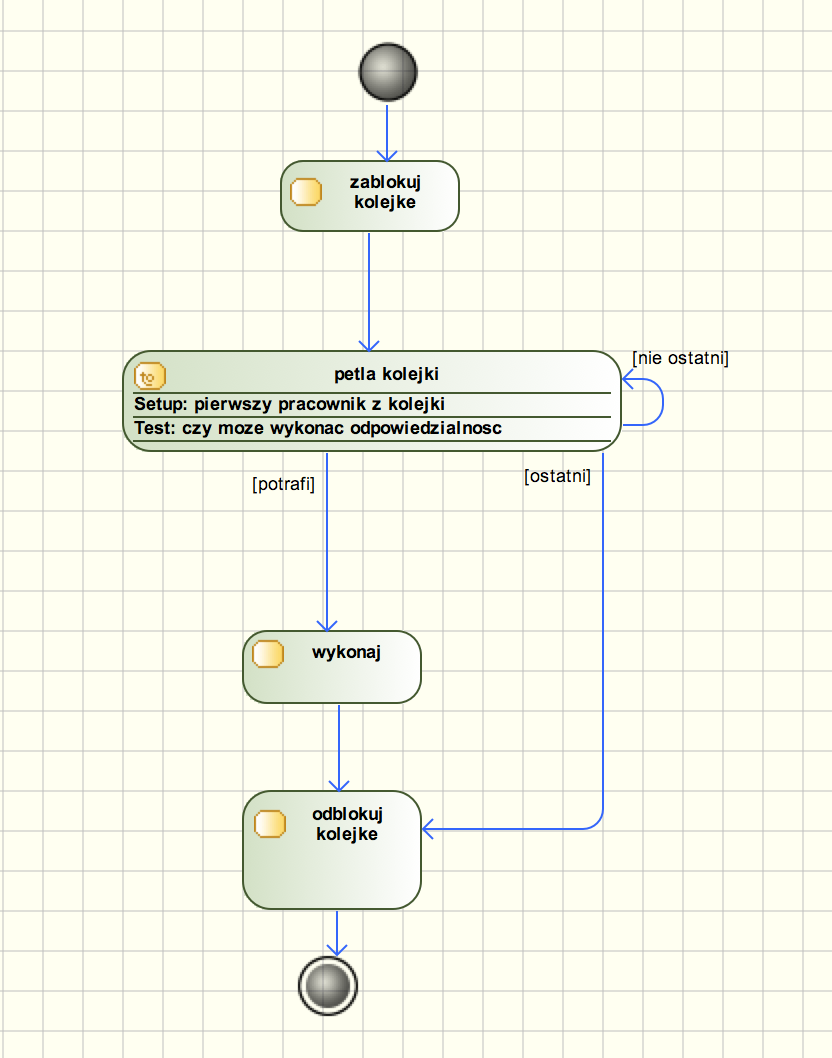
\includegraphics[width=\textwidth]{3}

Diagram dla AddWorker:

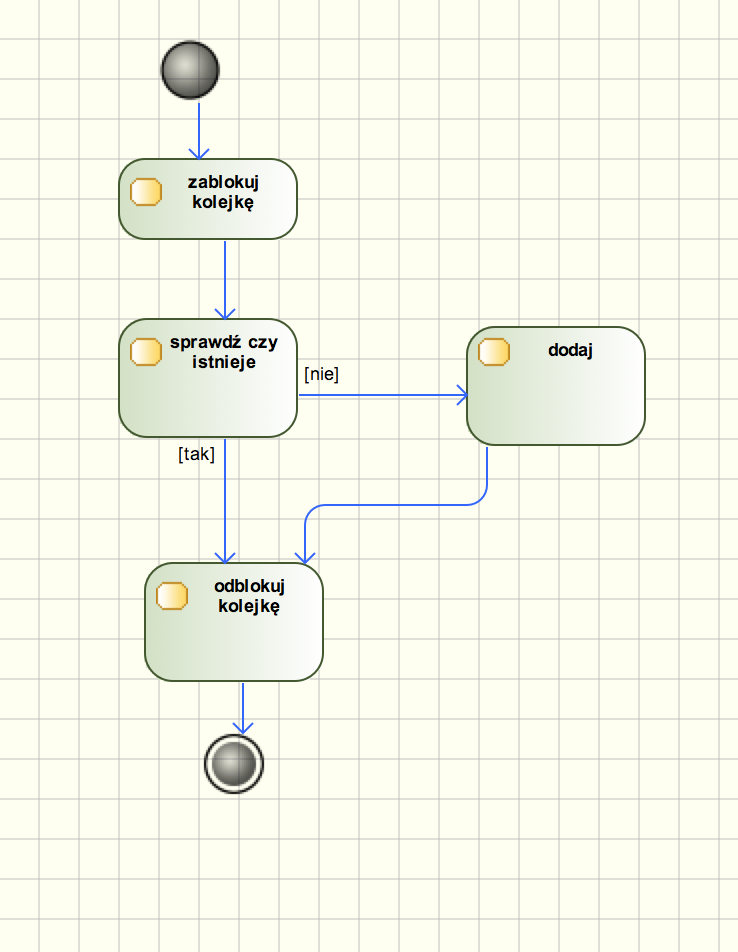
\includegraphics[width=\textwidth]{4}


Następnie po wyodrębnieniu scenariuszy zostało przetestowane przejście przez wszysktie przejścia w grafie.
Scenariusze zakładały:

\begin{itemize}
  \item Dodanie nowego Workera
  \item Próbę dodania Workera będącego w Kolejcę
  \item Próbę usunięcia istniejącego workera
  \item Próbę usunięcia nie istniejącego workera
  \item Próbe usunięcia workerów przy pomocy reamoveAllCapableWorker bez workerów spełniających kryterium 
  \item Próbe usunięcia workerów przy pomocy reamoveAllCapableWorker z workerami spełniających kryterium 
  \item Próbę wykonania execute przy braku odpowiedzialnego worera
  \item Próbę wykonania execute przy odpowiednim workerze 
  \item Próbę wykonania execute przy pustym łańcuchu 
\end{itemize}

\section{Wykonanie testów}

Testy zostały wykonane, odnotowano następujące błędy:
\begin{itemize}
  \item Brak możliwości usunięcia już dodanych wokerów bez przechowywania ich wskaźników
  \item Błąd przy wykonaniu funkcji execute przy pustym zbiorze workerów.
\end{itemize}


\section{Wnioski }

Podczas testów zauważonych zostało kilka błędów implementacji takich jak niezainicjalizowana prawidłowo lista.
Wykoanane testy biało skrzynkowe mimo niewielkiej skali problemu oraz małej bazy kodu zajeły znaczną część projektu.
Nie było możliwe przetestowanie integracyjne systemu ( składał się on jedynie z jednego modułu). W przyszłości 
możliwe jest dodanie klas fabryk workerów oraz chain of responsibility i przetestowanie integracyjne pomiędzy klasami.
Nawet w przypadku tak małej klasy ilość błędów wykrytych przy testowaniu jest dość duża.

\end{document}
